En este capítulo se detalla el proceso de desarrollo del proyecto. En primer lugar, se analizarán los requisitos del proyecto para definir la arquitectura general del sistema. Luego se describirán el análisis, el diseño y la complementación de los componentes. Por último, se mostrarán datos ofrecidos por las herramientas de soporte al desarrollo.
 
 
 desarrollo.
  
\section{Análisis de Requisitos}


En esta aplicación móvil para actividades a campo abierto objetivo de este proyecto, se establecieron una seria de requisitos generales que debería cumplir la aplicación.\\

El registro del usuario para poder comenzar a usarla.\\

La creación de puntos de interés marcados en un mapa con nombre, descripción y un punto en el mapa con o sin señal GPS clasificados en tipo, caza o pesca. \\

Se podrán guardar las rutas seguidas por un usuario en sus caminatas por cualquier tipo de terrero.\\

El usuario también podrá crear grupos con los usuarios que quiera y los integrantes del mismo poder añadir a otros, el resultado de esta funcionalidad es la que permitirá posteriormente  crear rutas conjuntas. Para crear una ruta conjunta primero se elige el grupo del que se hará el seguimiento y se enviarán  las invitaciones para participar en él a cada integrante del grupo. Estas invitaciones en el caso de ser aceptadas llevaran al usuario a un mapa y periódicamente se irán realizando actualizaciones de las posiciones del resto de integrantes del grupo anteriormente indicado. Finalmente se podrán ver las rutas conjuntas igual que las individuales.
\subsection{Actores}

Los únicos actores que se presentan en la  aplicación son los siguientes:
\begin{itemize}
\item \textbf{Usuario no  autenticado}.Usuario que no está autenticado en la aplicación y que
se le permite registrarse en el  sistema o iniciar sesión si la ya se registro en otro momento.
\item \textbf{Usuario  autenticado}.Usuario autenticado que puede acceder a todas as funcionalidades
del sistema.
\end{itemize}
\subsection{Casos de uso}
A continuación, en esta sección, se exponen los requisitos funcionales que surgen de los requisitos generales planteados en el punto anterior.
\subsubsection{• Usuario no autenticado}
\begin{itemize}
\item\textbf{ \textit{R1}  Registrarse en la aplicación.}
 El usuario podrá darse de alta en el sistema
introduciendo sus datos en el formulario que se le indican. Una vez registrado se iniciará sesión
automáticamente con el nuevo perfil.

\item \textbf{\textit{R2} Iniciar sesión en la aplicación. }
El usuario ya registrado podrá, con
sus credenciales, autenticarse en el  sistema. Se pedirá o nombre del usuario la aplicación y  su contraseña. Se guardará el estado en el terminal hasta que el usuario decida desconectarse.
\end{itemize} 
\begin{figure}[H]
		\centering
		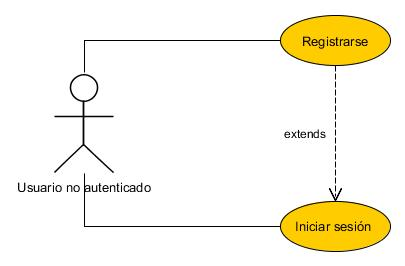
\includegraphics[width=0.75\textwidth] {usuario-no-autenticado.jpg}
		\caption{Casos de uso del actor Usuario No Autenticado }
	\end{figure}
\subsubsection{• Usuario  autenticado}
Para hacer un poco más comprensible dividiré los casos de uso del usuario autenticado por grupos funcionales.
\begin{itemize}
\item \textbf{Gestión de puntos de interés}\\
Aquí se describirán  los casos de uso relacionados con la gestión  de la  información del  los puntos de interés
\begin{itemize}
\item\textbf{\textit{ R-PDI-1 Guardar Punto De Interés caza}}, el usuario podrá guardar un punto concreto, de caza, asociado a un par de coordenadas pudiendo añadirle un nombre y una descripción.
\item\textit{ \textbf{R-PDI-2 Guardar Punto De Interés pesca}}, el caso de uno es similar al de anterior pero este es para el tipo de pesca.
\item \textbf{\textit{R-PDI-3 Eliminar PDI}}, el usuario podrá seleccionar un punto o una lista de puntos para ser borrados.
\item \textbf{\textit{R-PDI-4 Buscar los PDI}}, permite ver todos los puntos de interés de cada tipo por separado pintados en un mapa y pudiendo ciclar en ellos para conocer su nombre y descripción.
\end{itemize} 

\begin{figure}[H]
		\centering
		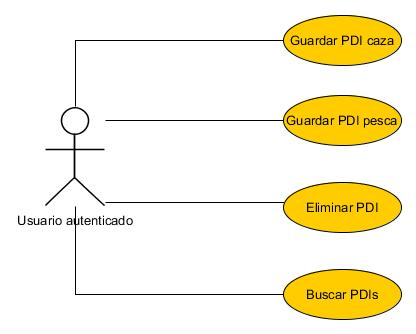
\includegraphics[width=0.75\textwidth] {PDI.jpg}
		\caption{Casos de uso de gestión de puntos de interés }
	\end{figure}
\item \textbf{Gestión de grupos}
\begin{itemize}
\item\textbf{ \textit{R-G-1 Crear grupo}}, el usuario crea un grupo con nombre único.
\item\textbf{\textit{ R-G-2 Añadir integrantes}}, el usuario busca en la base de datos los usuarios que quiere integrar en el grupo previamente creado.
\item \textbf{\textit{R-G-3 Eliminar integrantes}}, el usuario puede eliminar los integrantes que vea pertinentes.
\item \textbf{\textit{R-G-4 Ver grupos}}, el sistema listarla los grupos en los que el usuario está registrado.
\item \textbf{\textit{R-G-5 Ver integrantes grupo}}, el sistema permitirá ver los integrantes del grupo que el usuario indique , previo listado del caso de uso R-G-4. 

\end{itemize} 

\begin{figure}[H]
		\centering
		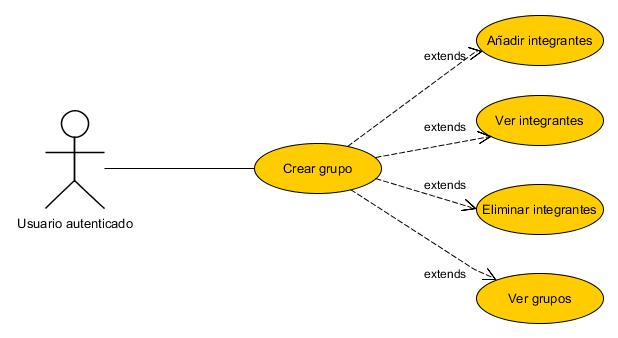
\includegraphics[width=0.75\textwidth] {grupo.jpg}
		\caption{Casos de uso de gestión de grupos de usuarios }
	\end{figure}
\item \textbf{Gestión de rutas,}el usuario iniciará una navegación privada siendo guardada la ruta seguida.
\begin{itemize}
\item \textbf\textit{{R-R-1 Crear ruta privada}}, el usuario registra la ruta con un nombre.
\begin{itemize}
\item \textbf{\textit{R-R-1.1}} Iniciar ruta, el sistema comienza a guardar las coordenadas por la que el usuario esta navegando y dibujando la ruta en el mapa. Las coordenadas se irán guardando periódicamente.
\item\textbf{ \textit{R-R-1.2}} Parar ruta, permite parar la navegación, tanto de guardar las coordenadas como de pintar la ruta seguida.
\item \textbf{\textit{R-R-1.3}} Guardar ruta, el sistema guarda los últimos puntos que quedaban sin actualizar y ejecuta el caso de uso ver ruta en el mapa(R-R-4).
\end{itemize}

\item \textbf{\textit{R-R-2 Crear ruta compartida}}, este caso de uso permite guardar la ruta seguida por el usuario y al mismo tiempo ver la posición del resto de integrantes de un grupo, anteriormente seleccionado, en tiempo real. Este caso de uso también enviaría a los integrantes del grupo una invitación a dicha ruta.
\begin{itemize}
\item \textbf{\textit{R-R-2.1 Iniciar ruta}}, se comienza a guardar y dibujar la ruta en el mapa. Por otra parte se comienza el seguimiento del resto de usuario que estén también navegando. Como también una actualización parcial de la ruta seguida en el servidor.
\item \textbf{\textit{R-R-2.2 Parar ruta}}, se para la navegación y se deja de actualizar la posición al resto de usuario de la ruta compartida.
\item \textbf{\textit{R-R-2.3 Finalizar ruta}}, se guardan los puntos que faltan de enviar al servidor y se deja de enviar datos al resto de integrantes.
\end{itemize}
\item \textbf{\textit{R-R-3 Listar rutas} }, permite al usuario ver todas las rutas realizadas tanto de manera privada como de manera compartida.
\item \textbf{\textit{R-R-4 Ver ruta en mapa}}, el sistema dibuja en un mapa la ruta seguida y previamente seleccionada.
\item \textbf{\textit{R-R-5 Eliminar ruta}}, permite al usuario borrar de la aplicación la ruta indicada.

\end{itemize} 
\end{itemize}
\begin{figure}[H]
		\centering
		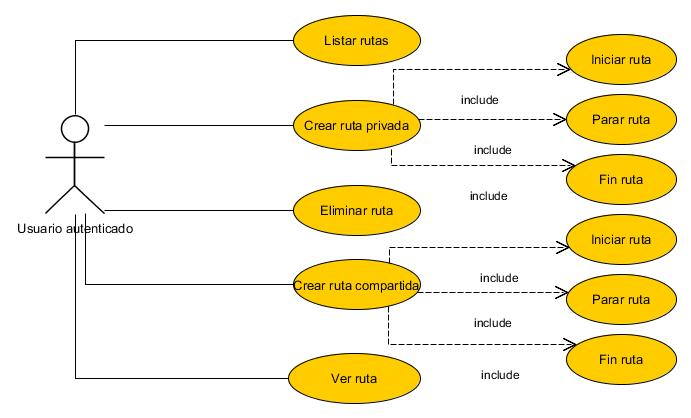
\includegraphics[width=0.75\textwidth] {rutas.jpg}
		\caption{Casos de uso de gestión de rutas }
	\end{figure}

\newpage
\section{Maquetas}
Comenzamos creando las maquetas de como debería que ser a interface del usuario.
Se busca que sea una interface simple y intuitiva.
Para esto, se intentarán seguir las pautas y usar lo  máximo posible los elementos de Material
Design [6].
Material Design es un lenguaje de diseñoo para distintas plataformas y dispositivos,
creada por el diseñador graco de Google Matas Duarte. Ofrece una guía  para ofrecer
a los usuarios una experiencia común y habitual entre distintas aplicaciones.


	
	
	
	\begin{figure}[htbp]
\begin{minipage}[b]{0.5\linewidth} %Una minipágina que cubre la mitad de la página
\centering
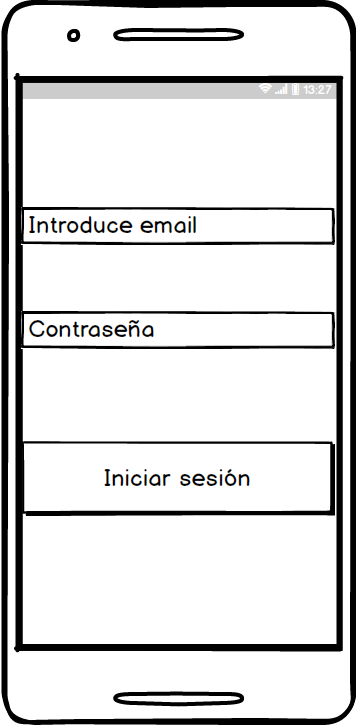
\includegraphics[width=6cm]{maqueta/Iniciar.png}
 \label{figura1}
\caption{Inisiar sesión}

\end{minipage}
\hspace{0.5cm} % Si queremos tener un poco de espacio entre las dos figuras
\begin{minipage}[b]{0.5\linewidth}
\centering
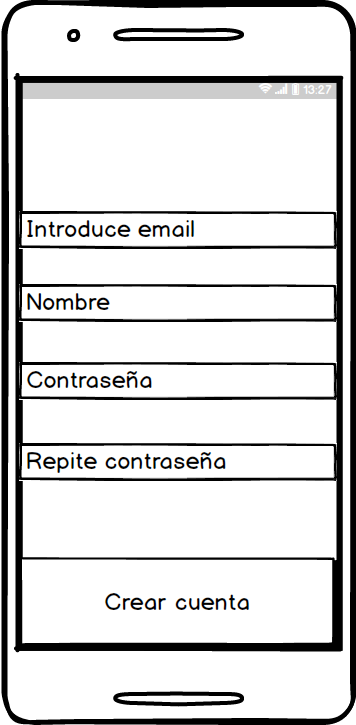
\includegraphics[width=6cm]{maqueta/Registrarse.png}
 \label{figura2}
\caption{Registrar usuario}

\end{minipage}
\end{figure}










	
	\begin{figure}[htbp]
\begin{minipage}[b]{0.5\linewidth} %Una minipágina que cubre la mitad de la página
\centering
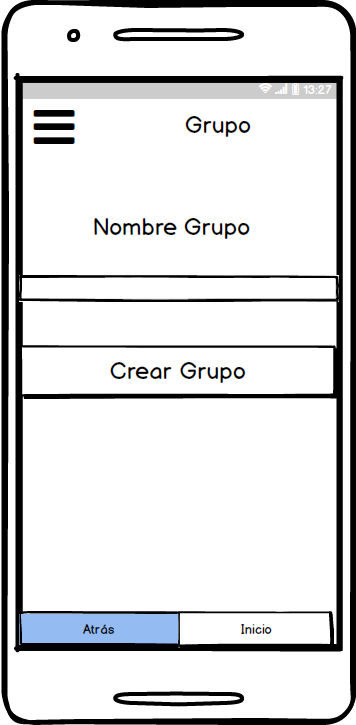
\includegraphics[width=6cm]{maqueta/Crear-Grupo.png}
 \label{figura1}
\caption{Crear grupo}

\end{minipage}
\hspace{0.5cm} % Si queremos tener un poco de espacio entre las dos figuras
\begin{minipage}[b]{0.5\linewidth}
\centering
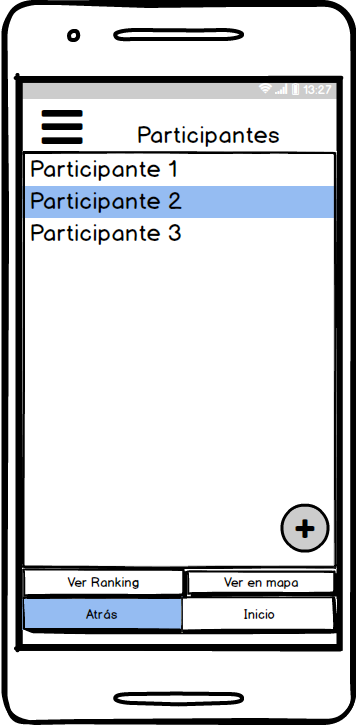
\includegraphics[width=6cm]{maqueta/Ver-Miembros-grupo.png}
 \label{figura2}
\caption{Añadir usuarios a grupo}

\end{minipage}
\end{figure}
	
	
	
	
	
	
	
	
	
	
	
	
	
	
	
	
	
	\begin{figure}[htbp]
\begin{minipage}[b]{0.5\linewidth} %Una minipágina que cubre la mitad de la página
\centering
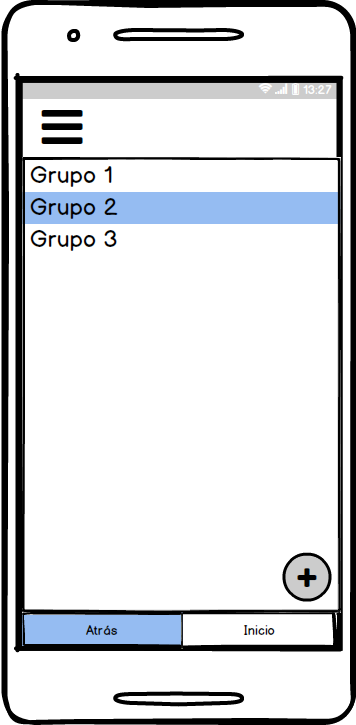
\includegraphics[width=6cm]{maqueta/lista-grupos.png}
 \label{figura1}
\caption{Listar grupos}

\end{minipage}
\hspace{0.5cm} % Si queremos tener un poco de espacio entre las dos figuras
\begin{minipage}[b]{0.5\linewidth}
\centering
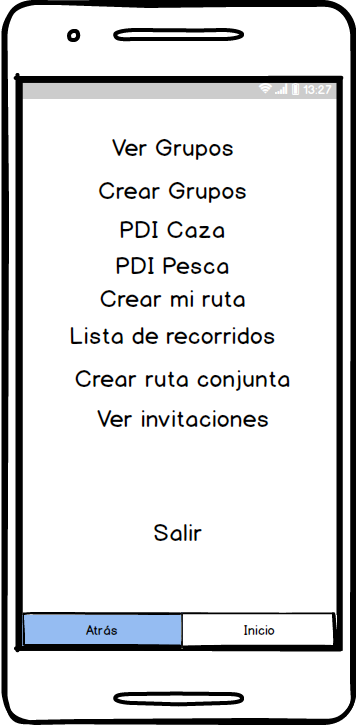
\includegraphics[width=6cm]{maqueta/opciones.png}
 \label{figura2}
\caption{Opciones generales}

\end{minipage}
\end{figure}
	















	\begin{figure}[htbp]
\begin{minipage}[b]{0.5\linewidth} %Una minipágina que cubre la mitad de la página
\centering
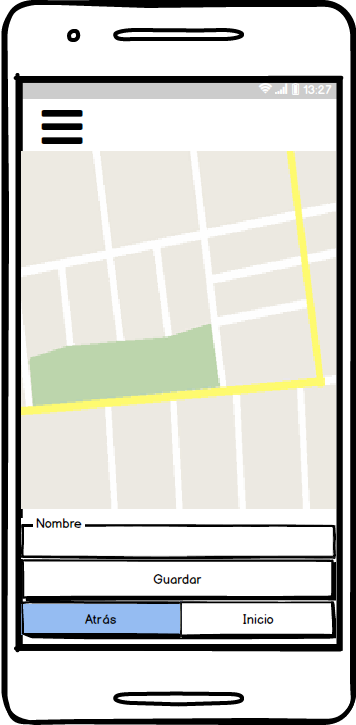
\includegraphics[width=6cm]{maqueta/pdi1.png}
 \label{figura1}
\caption{Crear PDI}

\end{minipage}
\hspace{0.5cm} % Si queremos tener un poco de espacio entre las dos figuras
\begin{minipage}[b]{0.5\linewidth}
\centering
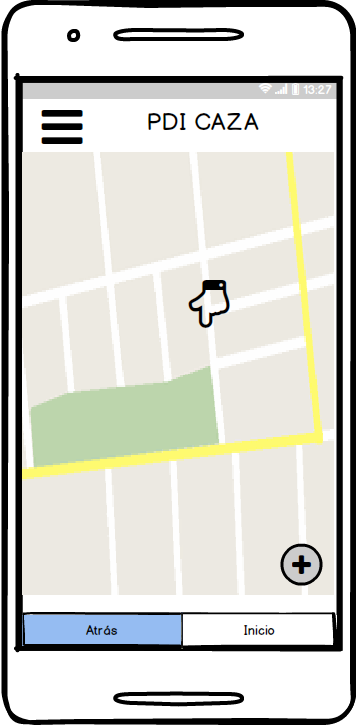
\includegraphics[width=6cm]{maqueta/pdi2.png}
 \label{figura2}
\caption{Visualizar PDIs}

\end{minipage}
\end{figure}
	

	\begin{figure}[htbp]
\begin{minipage}[b]{0.5\linewidth} %Una minipágina que cubre la mitad de la página
\centering
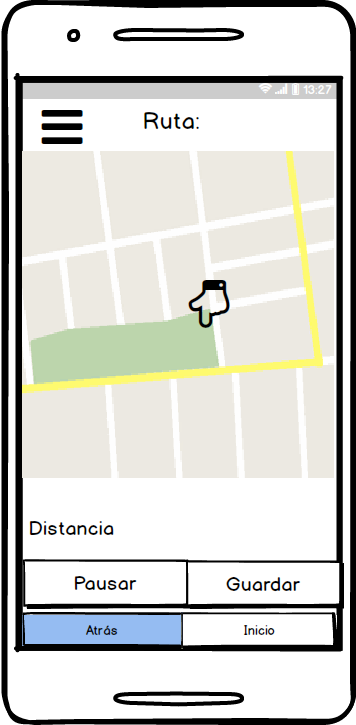
\includegraphics[width=6cm]{maqueta/Trayecto-actual.png}
 \label{figura1}
\caption{Ruta individual}

\end{minipage}
\hspace{0.5cm} % Si queremos tener un poco de espacio entre las dos figuras
\begin{minipage}[b]{0.5\linewidth}
\centering
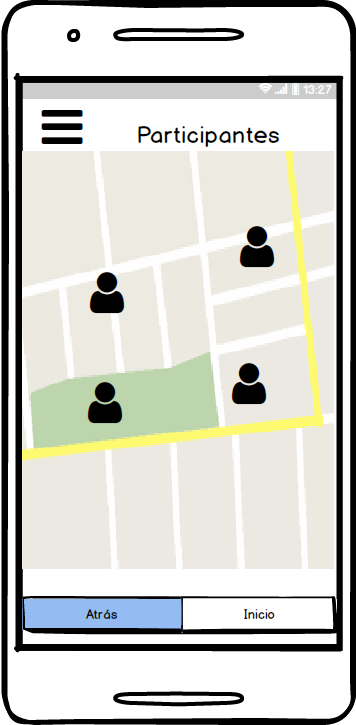
\includegraphics[width=6cm]{maqueta/Trayecto-actual-compartido.png}
 \label{figura2}
\caption{Ruta compartida}

\end{minipage}
\end{figure}



\newpage
\section{Arquitectura propuesta}
\label{s:dev:arch}
 

En este capítulo se comentará el diseño de la aplicación de manera superficial, la arquitectura general, el
modelo de datos y también aspectos más concretos del diseño del servidor y da aplicación
móvil.



\subsection{Arquitectura do sistema}
La aplicación que estamos desarrollando seguirá la arquitectura
en tres capas. Este patrón arquitectónico cliente/servidor se diferencian tres
capas, una capa de interface de usuario , una capa de persistencia
y una capa intermedia llamada de servicios que permite la llamada de forma remota a la capa modelo(capa que contiene la lógica) por parte del cliente Este patrón esta compuesto por:




\begin{figure}[H]
		\centering
		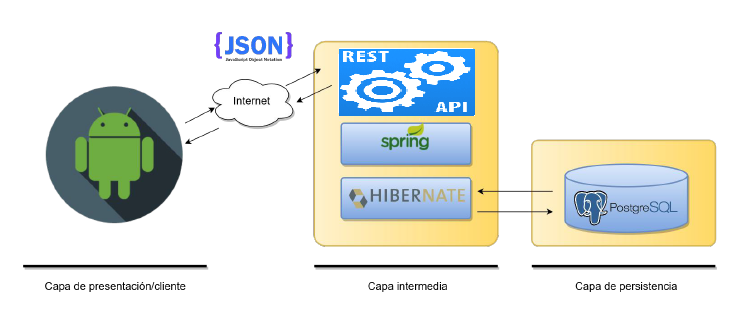
\includegraphics[width=0.75\textwidth] {arquitectura.png}
		\caption{Esquema general de la arquitectura del sistema }
	\end{figure}


\begin{itemize}
\item \textbf{Capa de presentación/cliente}:\\

A capa de presentacion mostra a informacion relacionada cos servizos prestados polo
sistema. Comuncase coas outras capas para obter e gardar os datos necesarios para
o usuario. Noutras palabras, e a capa que e empregada polo usuario.
\item \textbf{Capa intermedia:}\\


Esta capa e a encargada de enlazar a capa de persistencia coa capa cliente, e dicir,
de recoller os datos da nosa base de datos e envialos cara o cliente.
\item \textbf{Capa de persistencia:}\\


A capa de persistencia e a encargada de almacenar a informacion do sistema e
inclue unha capa de acceso a datos que encapsula os mecanismos de persistencia que
permiten o acceso os datos. Esta capa debe prover unha interface que posibilite a
comunicacion coa informacion almacenada pero sen expoñer ou crear dependencias
da tecnoloxa empregada no sistema de almacenamento. Desta forma permite crear
unha abstraccion do sistema a tecnoloxa empregada na base de datos para, logo,
ter unha maior 
exibilidade ante cambios ou actualizacions na tecnoloxa sen que as
demais capas se vexan afectadas.


\end{itemize}
En moitas ocasions, como e no caso que estamos a tratar, a capa intermedia pode estar
a sua vez tamen composta ou divida en varias capas propias. Podemos estar falando enton,
da as veces chamada arquitectura en N-capas.
Polo tanto o servidor segue o modelo Modelo-Vista-Controlador que consegue separar os
datos da aplicacion, a loxica de negocio da aplicacion e a transmision de informacion a rede.
Basease nas ideas de separacion de intereses e reutilizacion de codigo para as facilitar a
tarefa de desenvolvemento de aplicacions e o seu posterior mantemento.\\


Os componentes que forman parte do padron MVC son:

\begin{itemize}
\item \textbf{Modelo:}\\
Componse das clases que facilitan o acceso a datos ofrecendo unha serie de operacion
de mais alto nivel as capas superiores. Componse das entidades ou clases persistentes
mais un conxunto de clases que se encarga da sua xestion e unha fachada que ofrece
operacions as outras capas.
\item \textbf{vista:}\\
Esta formado pola interface na que ocorren as chamadas entre o servizo web e a
aplicacion cliente. O tratarse dun servizo web, unha serie de peticions HTTP comunicar
an a traves da internet informacion en formato JSON.

\item \textbf{controlador:}\\

E
o encargado de implementar a loxica da interface, invocando as operacions do
modelo e seleccionando a vista encargada de cada peticion.



\end{itemize}




\subsection{Diagrama de despliegue}
Una vez creada la arquitectura, hay que determinar las elecciones tecnológicas que dan soporte a la misma. Dicho estudio se encuentra recogido en el Capítulo~\ref{s:tech}. La configuración del despliegue de la aplicación se recoge en la Figura~\ref{f:dev:arch-deploy}.

\begin{figure}[h!]
\centering
%\includegraphics[width=1.1\textwidth]{img/deploy}
\caption{Diagrama de despliegue del sistema}
\label{f:dev:arch-deploy}
\end{figure}


\section{Componente A}
En esta sección se estudiará el componente A...

\subsection{Análisis}
Este componente del sistema da respuesta al requisito <<R? xxx>> 

\subsubsection{Casos de uso}
En base a los requisitos educidos, se exponen los casos de uso de este subsistema.

En la Figura~\ref{f:dev:use-cases-recsys} se ilustra el diagrama de casos de uso correspondiente al componente A.

\begin{figure}[h!]
\centering
%\includegraphics[width=\textwidth]{img/use-cases-compA}
\caption{Diagrama de casos de uso relativos al componente A}
\label{f:dev:use-cases-recsys}
\end{figure}

\subsubsection{Modelo de datos}


\subsection{Diseño e implementación}
En esta sección se presenta el diseño seguido para implementar el motor de recomendación. Se empleará el lenguaje de modelado UML para ilustrar la estructura de este subsistema.
